\chapter{Engenharia genética e biotecnologia}\label{ch:b3:genetic-engineering}

Até 1982 todo diabético do mundo era mantido vivo por insulina
extraída do pâncreas de porcos e de bois --- umas oito mil toneladas de
glândulas para cada tonelada de hormônio, na mesma proporção --- e uma
fração dos pacientes reagia contra a proteína estranha. Naquele ano
chegou ao mercado o primeiro fármaco feito por um organismo
geneticamente modificado: a insulina humana, sintetizada por
\emph{Escherichia coli} que carregava o gene humano num \omterm{def:b3:genetic-engineering:tools}{plasmídeo}. As
ferramentas que tornaram isso possível haviam sido reunidas na década
anterior --- enzimas que cortam o DNA em sequências escolhidas, enzimas
que unem os pedaços, \omterm{def:b3:genetic-engineering:tools}{plasmídeos} que os levam para dentro de uma célula
e os copiam ali --- e a elas se juntaram, nas décadas seguintes, a
\omterm{def:b3:genetic-engineering:pcr}{reação em cadeia da polimerase}, a injeção de genes em embriões e,
desde 2012, um sistema imune bacteriano transformado numa tesoura
programável capaz de reescrever uma letra de um genoma numa célula
viva. Este capítulo trata dessas ferramentas, da aritmética que rege
seu uso e do que já se construiu com elas, de um camundongo que brilha
a uma cura para a doença falciforme.

\section{Cortar, unir e copiar DNA}

\begin{definition}[Enzimas de restrição, ligase e vetores]\label{def:b3:genetic-engineering:tools}
\index{enzima de restrição}\index{extremidade coesiva}\index{DNA-ligase}\index{vetor}\index{plasmídeo}\index{marcador de seleção}
Uma \emph{enzima de restrição} do tipo~II é uma endonuclease bacteriana
que corta o DNA de fita dupla numa sequência específica de
\numrange{4}{8} pares de bases, em geral um palíndromo: a EcoRI corta
G$^{\downarrow}$AATTC, deixando saliências de fita simples de quatro
bases (\emph{extremidades coesivas}) complementares a qualquer outra
extremidade EcoRI; outras enzimas deixam \emph{extremidades cegas}. A
\emph{DNA-ligase} sela dois fragmentos cujas extremidades se encaixam.
Um \emph{vetor} é uma molécula de DNA que se replica num hospedeiro e
pode carregar um fragmento inserido: um \emph{plasmídeo} de algumas
quilobases com uma origem de replicação, um \emph{marcador de seleção}
(um gene de resistência a antibiótico, de modo que só as células que
receberam o plasmídeo crescem no antibiótico) e um agrupamento de
sítios de restrição únicos para o inserto; o bacteriófago $\lambda$,
cosmídeos e cromossomos artificiais de bactéria ou de levedura para
insertos de \qtyrange{20}{1000}{kb}. O DNA entra numa bactéria por
\emph{transformação}, depois de um choque químico ou elétrico que torna
a membrana transitoriamente permeável, com eficiência de $10^{6}$ a
$10^{9}$ transformantes por micrograma de plasmídeo. Uma molécula
\emph{recombinante} é a que une DNA de duas fontes.
\end{definition}

\begin{proof}[Evidência]
Cohen, Chang, Boyer e Helling (1973) cortaram com EcoRI o \omterm{def:b3:genetic-engineering:tools}{plasmídeo}
pSC101 e um segundo \omterm{def:b3:genetic-engineering:tools}{plasmídeo} que carregava outro gene de resistência,
misturaram e ligaram os fragmentos, transformaram \emph{E.~coli} e
recuperaram colônias resistentes aos dois antibióticos, que carregavam
um único \omterm{def:b3:genetic-engineering:tools}{plasmídeo} feito dos dois --- o primeiro DNA recombinante a se
replicar numa célula. No ano seguinte inseriram genes de RNA
ribossômico de um sapo no pSC101 e mostraram que o DNA do anfíbio era
replicado, e transcrito, na bactéria: os genes cruzam a fronteira entre
os reinos sem mudar, e uma bactéria copia qualquer DNA que lhe deem.
\end{proof}

\begin{omfigure}
\begin{tikzpicture}[every node/.style={font=\scriptsize}, >=stealth]
  % plasmid circle
  \draw[very thick, omDef] (0,0) circle (1.8);
  % ori
  \draw[very thick, omMeth!70!black] (0,0) ++(60:1.8) arc[start angle=60, end angle=100, radius=1.8]; \node[above right] at (80:1.95) {origem de replicação};
  % ampR
  \draw[very thick, omProp] (0,0) ++(160:1.8) arc[start angle=160, end angle=250, radius=1.8]; \node[left, align=right] at (205:2.0) {gene de\\resistência\\(marcador)};
  % MCS with insert
  \draw[very thick, omThm] (0,0) ++(-40:1.8) arc[start angle=-40, end angle=10, radius=1.8]; \node[right, align=left] at (-15:2.0) {inserto, ligado ao\\sítio de restrição};
  \draw[omThm] (-40:1.7) -- (-40:1.95); \draw[omThm] (10:1.7) -- (10:1.95);
  \node at (0,0.25) {plasmídeo}; \node at (0,-0.15) {\qtyrange{3}{5}{kb}};
  % sticky ends detail
  \begin{scope}[xshift=5.7cm, yshift=0.8cm]
    \node[left, align=right] at (-0.2,0) {EcoRI};
    \node[font=\ttfamily\scriptsize, anchor=west] at (0,0.25) {5$'$-G\,\textcolor{omThm}{AATT}C-3$'$};
    \node[font=\ttfamily\scriptsize, anchor=west] at (0,-0.25) {3$'$-C\textcolor{omThm}{TTAA}\,G-5$'$};
    \draw[->, omThm, thick] (0.62,0.55) -- (0.62,0.3); \draw[->, omThm, thick] (1.62,-0.55) -- (1.62,-0.3);
    \node[anchor=west, align=left] at (2.9,0) {cortes escalonados\\deixam saliências\\complementares de quatro\\bases: pontas coesivas};
  \end{scope}
  \begin{scope}[xshift=5.7cm, yshift=-1.3cm]
    \draw[very thick, omDef] (0,0.15) -- (1.2,0.15); \draw[very thick, omDef] (0,-0.15) -- (0.7,-0.15);
    \draw[very thick, omThm] (1.7,0.15) -- (3.0,0.15); \draw[very thick, omThm] (1.2,-0.15) -- (3.0,-0.15);
    \node[above] at (1.45,0.2) {anelar}; \node[below, align=center] at (1.5,-0.25) {quaisquer duas pontas EcoRI\\pareiam; a ligase sela\\o esqueleto};
  \end{scope}
\end{tikzpicture}

{\small Um \omterm{def:b3:genetic-engineering:tools}{vetor} de clonagem e sua química. O \omterm{def:b3:genetic-engineering:tools}{plasmídeo} carrega uma
origem, um \omterm{def:b3:genetic-engineering:tools}{marcador de seleção} e um sítio de restrição único ao qual se
liga um fragmento cortado pela mesma enzima; as \omterm{def:b3:genetic-engineering:tools}{extremidades coesivas}
tornam compatíveis dois fragmentos quaisquer cortados pela mesma
enzima.}
\end{omfigure}

\begin{method}[Clonar um gene]\label{met:b3:genetic-engineering:cloning}
\index{clonagem}\index{biblioteca}\index{triagem}
(1) Obtenha o inserto: corte o DNA genômico com uma \omterm{def:b3:genetic-engineering:tools}{enzima de
restrição}, ou copie o RNA mensageiro em DNA complementar (cDNA, que não
tem íntrons e por isso pode ser expresso em bactérias), ou amplifique o
gene por PCR com \omterm{def:b3:genetic-engineering:pcr}{iniciadores} que carregam sítios de restrição. (2)
Corte o \omterm{def:b3:genetic-engineering:tools}{vetor} e o inserto com a(s) mesma(s) enzima(s) --- duas enzimas
diferentes forçam a orientação do inserto --- e ligue-os. (3)
Transforme bactérias e plaqueie no antibiótico: só as células com
\omterm{def:b3:genetic-engineering:tools}{plasmídeo} crescem. (4) Distinga os \omterm{def:b3:genetic-engineering:tools}{plasmídeos} com inserto dos que se
fecharam sobre si mesmos: um gene marcador interrompido pelo sítio de
clonagem (\emph{lacZ}: as colônias brancas têm inserto, as azuis não).
(5) Faça a triagem das colônias em busca do inserto desejado: por
hibridação com uma sonda marcada, por PCR, ou por digestão com \omterm{def:b3:genetic-engineering:tools}{enzimas
de restrição} e eletroforese em gel. (6) Sequencie o inserto. Uma
\emph{biblioteca} é a coleção de clones de um genoma ou transcriptoma
inteiro, da qual qualquer gene pode ser pescado pela mesma triagem.
\end{method}

\begin{omfigure}
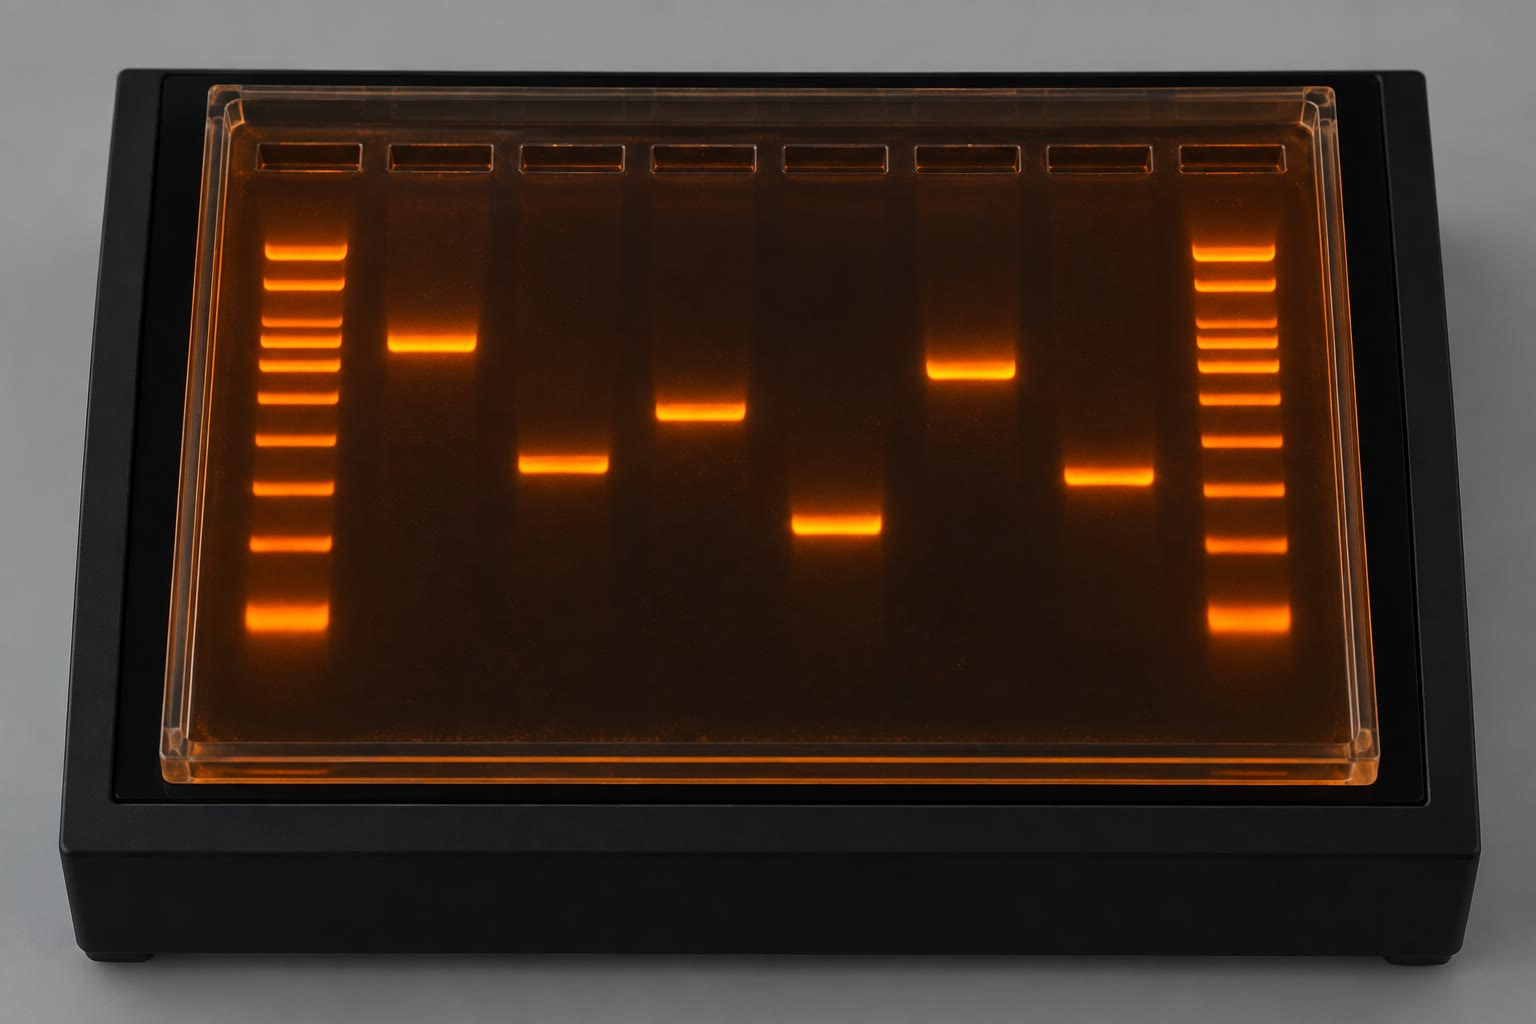
\includegraphics[width=0.56\linewidth]{images/book5/ai/b5-06-agarose-gel.jpg}

{\small Um gel de agarose sob luz ultravioleta: os fragmentos de DNA
migram rumo ao ânodo a uma velocidade que cai com o comprimento deles,
de modo que cada banda é uma população de moléculas de um mesmo
tamanho, comparada com a escada de tamanhos conhecidos nas raias
externas.}
\end{omfigure}

\begin{definition}[A reação em cadeia da polimerase]\label{def:b3:genetic-engineering:pcr}
\index{reação em cadeia da polimerase}\index{iniciador}\index{PCR quantitativa}
A \emph{reação em cadeia da polimerase} (PCR) amplifica um trecho
escolhido de DNA entre dois \emph{iniciadores} --- oligonucleotídeos
sintéticos de cerca de vinte bases complementares às duas fitas nas
extremidades do alvo --- por ciclos de três temperaturas:
\qty{95}{\celsius} para separar as fitas,
\qtyrange{50}{65}{\celsius} para os iniciadores anelarem,
\qty{72}{\celsius} para uma polimerase termoestável (a Taq, da bactéria
de fontes termais \emph{Thermus aquaticus}) estendê-los. Cada ciclo
dobra o número de cópias do segmento entre os iniciadores, de modo que
trinta ciclos convertem uma única molécula em um bilhão. A \emph{PCR de
transcrição reversa} primeiro copia o RNA em DNA e assim mede
transcritos ou vírus de RNA; a \emph{PCR quantitativa} (qPCR) acompanha
a amplificação em tempo real com um corante fluorescente e lê a
quantidade inicial a partir do ciclo em que o sinal cruza um limiar.
\end{definition}

\begin{theorem}[A aritmética da amplificação]\label{thm:b3:genetic-engineering:pcr}
\index{ciclo limiar}
Com eficiência $E$ por ciclo ($E = 1$ para uma duplicação perfeita),
$N_{0}$ cópias iniciais se tornam
\[
N_{n} = N_{0}\,(1 + E)^{n}
\]
após $n$ ciclos. Se a fluorescência cruza um limiar fixo quando o
número de cópias alcança $N_{T}$, o \emph{\omterm{thm:b3:genetic-engineering:pcr}{ciclo limiar}} é
\[
C_{T} = \frac{\log N_{T} - \log N_{0}}{\log(1 + E)},
\]
uma reta em $\log N_{0}$ com inclinação $-1/\log(1+E)$: para $E = 1$,
cada aumento de dez vezes na quantidade inicial baixa o $C_{T}$ em
$\log_{2} 10 = 3.32$ ciclos, e duas amostras cujos \omterm{thm:b3:genetic-engineering:pcr}{ciclos limiares}
diferem de $\Delta C_{T}$ diferem em cópias iniciais pelo fator
$(1 + E)^{\Delta C_{T}}$.
\end{theorem}
\begin{proof}
Cada ciclo multiplica o número de cópias por $1 + E$, de modo que
$N_{n}$ é uma progressão geométrica. Fazendo $N_{n} = N_{T}$ e
resolvendo para $n$ obtém-se $C_{T}$; a inclinação é o coeficiente de
$\log N_{0}$. Para duas amostras, $C_{T,1} - C_{T,2} = (\log N_{0,2} - \log N_{0,1})/\log(1+E)$, de onde $N_{0,2}/N_{0,1} = (1+E)^{\Delta C_{T}}$.
\end{proof}

\begin{example}[Ler uma placa de qPCR]\label{ex:b3:genetic-engineering:qpcr}
Um teste de RNA viral cruza o limiar no ciclo $22$ num paciente e no
ciclo $32$ em outro; com $E \approx 1$ o primeiro carrega $2^{10}
\approx 1000$ vezes mais vírus. Uma amostra de dez cópias cruza por
volta do ciclo $37$ quando o limiar é de $10^{12}$ cópias
($\log_{2} 10^{11} =
36.5$); uma corrida de $40$ ciclos detecta,
portanto, algumas poucas moléculas --- e uma única molécula
contaminante de um amplicon anterior também é detectada, e é por isso
que os laboratórios separam as salas onde a PCR é montada daquelas em
que os produtos são manipulados.
\end{example}

\begin{omfigure}
\begin{tikzpicture}
\begin{axis}[
  width=0.7\linewidth, height=5.6cm,
  axis x line=bottom, axis y line=left,
  xmin=0, xmax=40, ymin=1, ymax=1e14, ymode=log,
  xlabel={ciclo}, ylabel={cópias},
  xlabel style={font=\small, at={(axis description cs:0.5,-0.12)}, anchor=north},
  ylabel style={font=\small},
  tick label style={font=\small}, xtick={0,10,20,30,40},
  clip=false,
]
\addplot[very thick, omDef, domain=0:40, samples=41] {1e7*2^x/(1+2^x/1e5)};
\addplot[very thick, omThm, domain=0:40, samples=41] {1e4*2^x/(1+2^x/1e8)};
\addplot[very thick, omMeth!70!black, domain=0:40, samples=41] {10*2^x/(1+2^x/1e11)};
\addplot[dashed, gray, domain=0:40, samples=2] {1e12};
\node[font=\scriptsize, gray, anchor=south west] at (axis cs:0.5,1.3e12) {limiar $N_{T}$};
\draw[gray] (axis cs:16.6,1) -- (axis cs:16.6,1e12); \draw[gray] (axis cs:26.6,1) -- (axis cs:26.6,1e12); \draw[gray] (axis cs:36.5,1) -- (axis cs:36.5,1e12);
\node[font=\scriptsize, anchor=south] at (axis cs:16.6,3e12) {$C_{T} = 16.6$}; \node[font=\scriptsize, anchor=south] at (axis cs:26.6,3e12) {$26.6$}; \node[font=\scriptsize, anchor=south] at (axis cs:36.5,3e12) {$36.5$};
\end{axis}
\end{tikzpicture}

{\small Curvas de amplificação para $N_{0} = 10^{7}$ (azul), $10^{4}$
(vermelho) e $10$ cópias (verde), $E = 1$, com o platô que os reagentes
impõem. Uma diferença de mil vezes em $N_{0}$ desloca o \omterm{thm:b3:genetic-engineering:pcr}{ciclo limiar} em
$10$; os platôs são todos parecidos, e é por isso que o produto final
nada diz sobre o início.}
\end{omfigure}

\section{Fazer proteínas}

\begin{definition}[Sistemas de expressão]\label{def:b3:genetic-engineering:expression}
\index{vetor de expressão}\index{proteína recombinante}\index{anticorpo monoclonal}
Um \emph{\omterm{def:b3:genetic-engineering:tools}{vetor} de expressão} põe a sequência codificadora clonada sob
um promotor forte e controlável do hospedeiro (o promotor \emph{lac} ou
o T7 em \emph{E.~coli}, induzidos por um análogo de açúcar), com um
sítio de ligação ao ribossomo, um terminador e, muitas vezes, uma
\emph{etiqueta} --- seis histidinas, uma pequena proteína --- fundida ao
produto para purificação numa coluna. As bactérias produzem gramas por
litro de uma proteína simples (insulina, hormônio de crescimento,
enzimas), mas não conseguem glicosilar nem enovelar proteínas de
mamífero complexas; a levedura acrescenta açúcares à sua própria
maneira; células de inseto e de mamífero (as células de ovário de
hamster chinês são o padrão da indústria) produzem anticorpos e fatores
de coagulação enovelados e glicosilados como num humano. Um
\emph{anticorpo monoclonal} é feito por um \emph{hibridoma} --- um
linfócito~B produtor de anticorpo fundido a uma célula imortal de
mieloma (Köhler e Milstein, 1975) --- ou, hoje, clonando os genes do
anticorpo numa linhagem de expressão de mamífero, em que o arcabouço
murino pode ser substituído por sequência humana para evitar a rejeição
imune (\cref{ch:b3:adaptive-immunity}).
\end{definition}

\begin{example}[Insulina]\label{ex:b3:genetic-engineering:insulin}
A insulina humana são duas cadeias, a A (21 resíduos) e a B (30),
unidas por pontes dissulfeto e recortadas na célula~$\beta$ a partir de
um único precursor, a pró-insulina. O primeiro processo expressava as
duas cadeias separadamente em \emph{E.~coli}, cada uma fundida à
$\beta$-galactosidase, clivava-as quimicamente e as unia in vitro; os
processos posteriores expressam a pró-insulina e a clivam com as
enzimas que o pâncreas usa. Desde 1996 a própria sequência vem sendo
alterada: trocar ou acrescentar um resíduo ou dois dá análogos que se
dissociam mais depressa (para uma refeição) ou que precipitam no local
da injeção e se liberam ao longo de um dia. Uma proteína que exigia
oito toneladas de glândulas por quilograma é hoje feita num
fermentador, idêntica à humana ou melhor que ela.
\end{example}

\section{Organismos transgênicos}

\begin{definition}[Transgênese e direcionamento gênico]\label{def:b3:genetic-engineering:transgenic}
\index{organismo transgênico}\index{microinjeção}\index{nocaute}\index{célula-tronco embrionária}\index{direcionamento gênico}
Um organismo \emph{transgênico} carrega um gene introduzido em sua
linhagem germinativa, de modo que toda célula o tem e ele é herdado.
Nos camundongos a via clássica é a \emph{microinjeção} do DNA num dos
pronúcleos de um óvulo fecundado (Gordon e Ruddle, 1980), que se
integra num sítio aleatório numa fração dos embriões; Palmiter e
Brinster (1982) produziram camundongos do dobro do tamanho normal
injetando o gene do hormônio de crescimento de rato atrás de um
promotor de metalotioneína. O \emph{direcionamento gênico} substitui ou
rompe um gene escolhido: uma construção com braços longos homólogos ao
alvo é introduzida em \emph{células-tronco embrionárias}, as raras
células em que a \omterm{def:b3:dna-repair:dsb}{recombinação homóloga} a pôs no lugar certo são
selecionadas e injetadas num blastocisto, e o camundongo quimérico que
daí resulta transmite o gene alterado (Capecchi, Smithies e Evans,
anos 1980). Um \emph{nocaute} não tem o gene; um \emph{knock-in}
carrega uma versão modificada; um alelo \emph{condicional}, ladeado por
sítios loxP, é deletado só onde e quando a Cre é expressa
(\cref{ch:b3:dna-repair}). Uns dez mil genes de camundongo já foram
nocauteados e, para a maioria, o fenótipo foi a primeira indicação do
que o gene faz.
\end{definition}

\begin{omfigure}
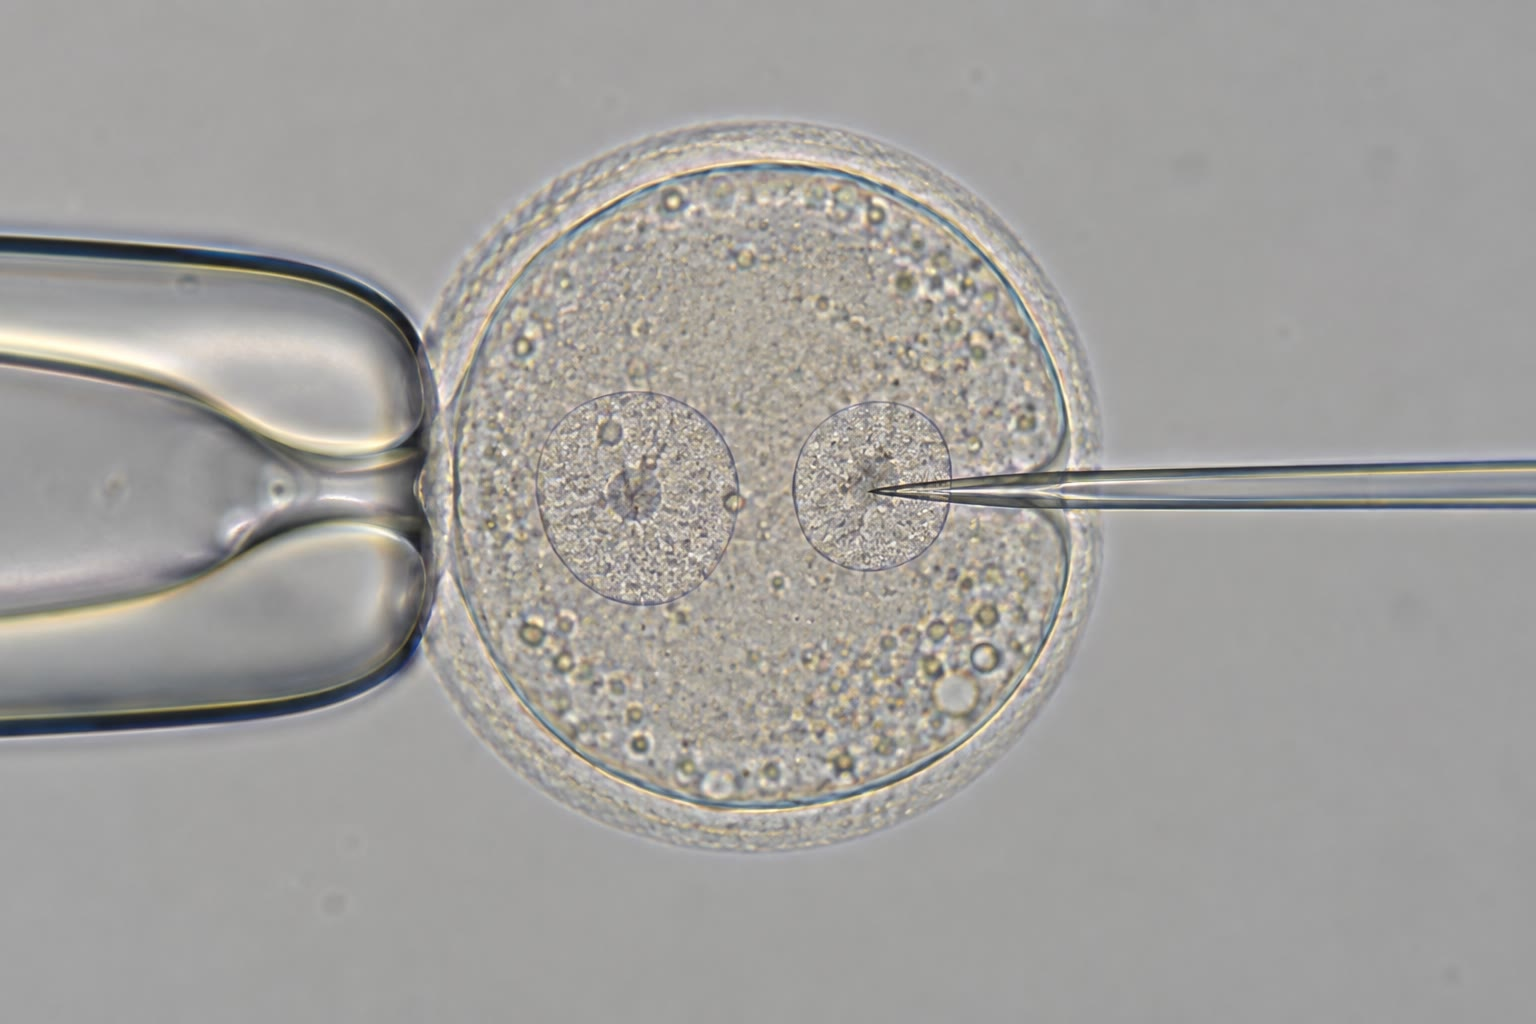
\includegraphics[width=0.46\linewidth]{images/book5/ai/b5-06-microinjection.jpg}\hspace{0.04\linewidth}
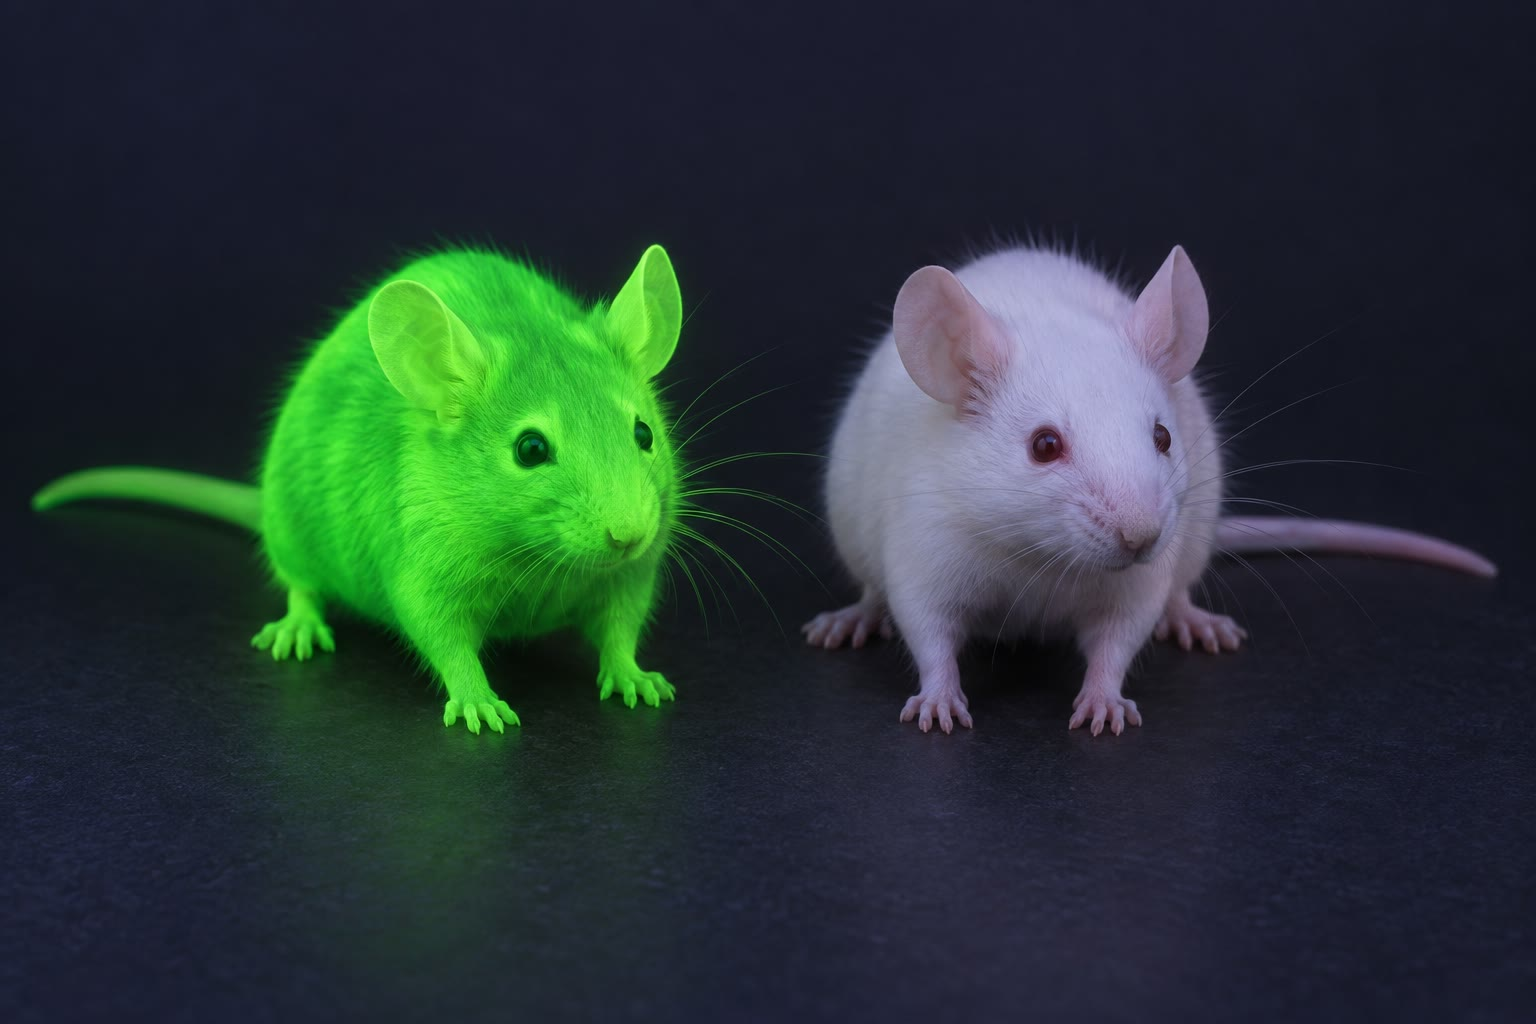
\includegraphics[width=0.46\linewidth]{images/book5/ai/b5-06-gfp-mouse.jpg}

{\small À esquerda: um óvulo de camundongo fecundado, segurado por
sucção enquanto uma agulha de vidro injeta DNA num dos pronúcleos. À
direita: um camundongo \omterm{def:b3:genetic-engineering:transgenic}{transgênico} que expressa em cada célula a
proteína fluorescente verde de uma água-viva, ao lado de um irmão de
ninhada comum, sob luz ultravioleta.}
\end{omfigure}

\begin{definition}[Plantas transgênicas]\label{def:b3:genetic-engineering:plants}
\index{Agrobacterium}\index{T-DNA}\index{cultivo geneticamente modificado}
As plantas são transformadas por \emph{Agrobacterium tumefaciens}, uma
bactéria do solo que naturalmente insere um segmento de seu \omterm{def:b3:genetic-engineering:tools}{plasmídeo}
indutor de tumor, o \emph{T-DNA}, no genoma de uma planta ferida, para
fazê-la produzir uma galha e alimentar a bactéria. Substituir os
próprios genes do T-DNA por qualquer gene de escolha, entre as
sequências de borda que a bactéria reconhece, converte o patógeno num
\omterm{def:b3:genetic-engineering:tools}{vetor}; as células transformadas são selecionadas e regeneradas em
plantas inteiras, coisa que qualquer célula vegetal sabe fazer. As
espécies que a bactéria não infecta (os cereais, por muito tempo) são
transformadas disparando partículas de ouro recobertas de DNA no
tecido. Os \emph{cultivos geneticamente modificados} plantados em
escala carregam um gene de toxina bacteriana (\emph{Bt}) contra larvas
de insetos, ou uma enzima bacteriana que confere tolerância a um
herbicida, ou os dois; o \emph{Arroz Dourado} carrega dois genes da via
dos carotenoides (uma fitoeno-sintase vegetal e uma dessaturase
bacteriana) para que seu endosperma produza $\beta$-caroteno, o
precursor da vitamina~A, cuja deficiência cega e mata várias centenas
de milhares de crianças por ano.
\end{definition}

\begin{omfigure}
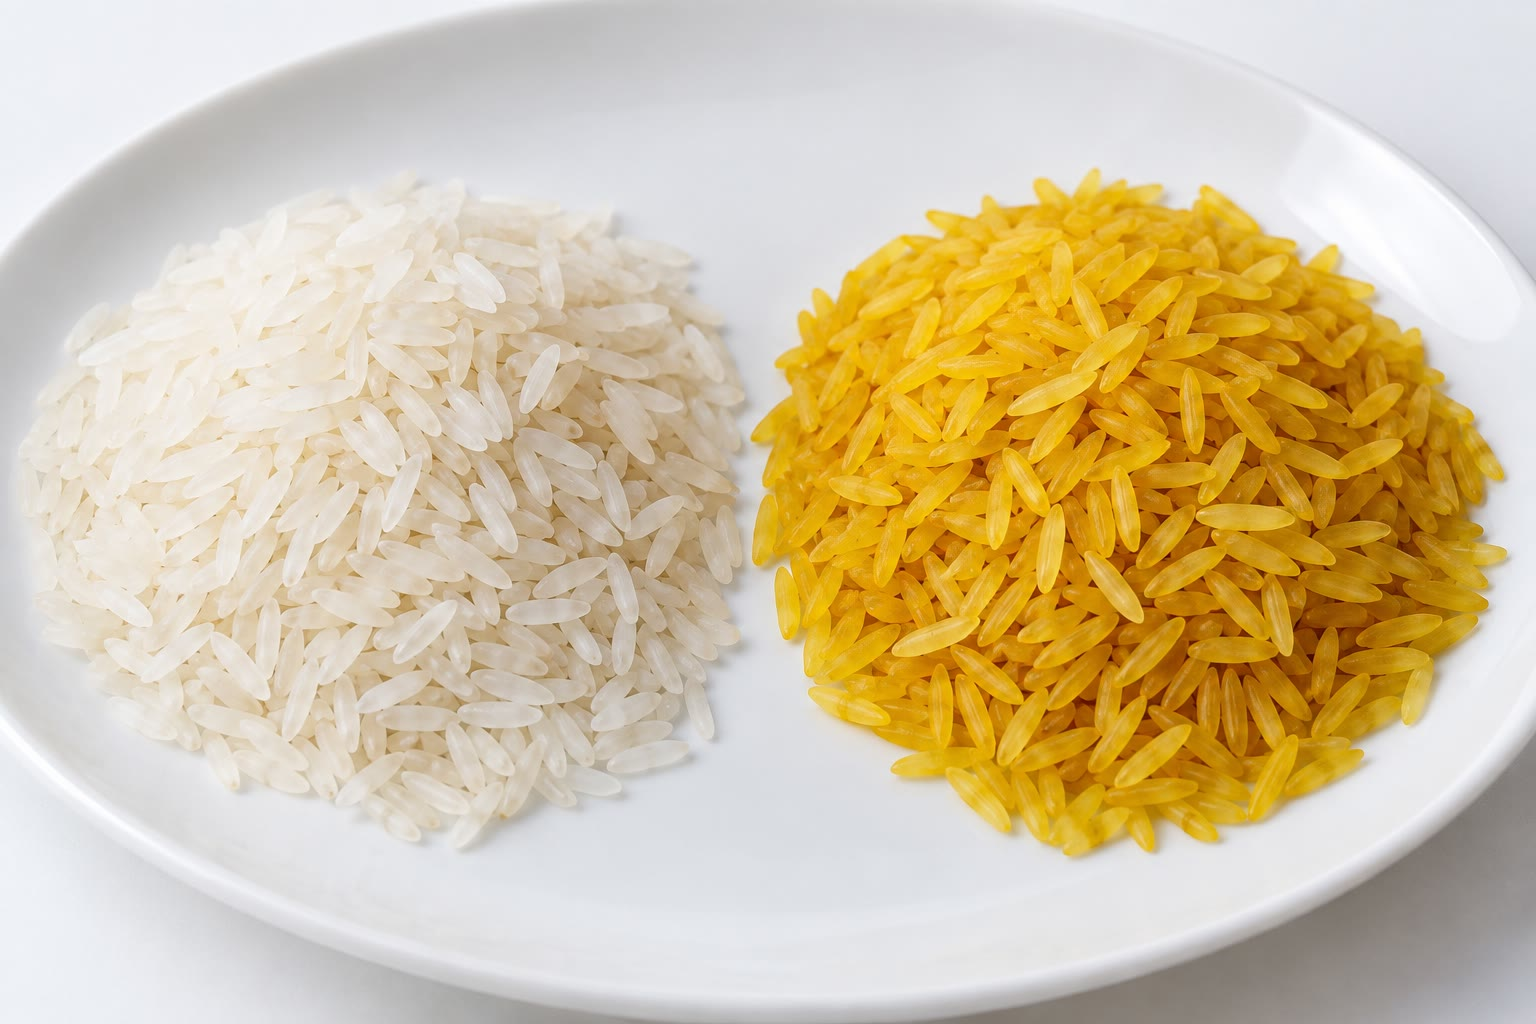
\includegraphics[width=0.46\linewidth]{images/book5/ai/b5-06-golden-rice.jpg}\hspace{0.04\linewidth}
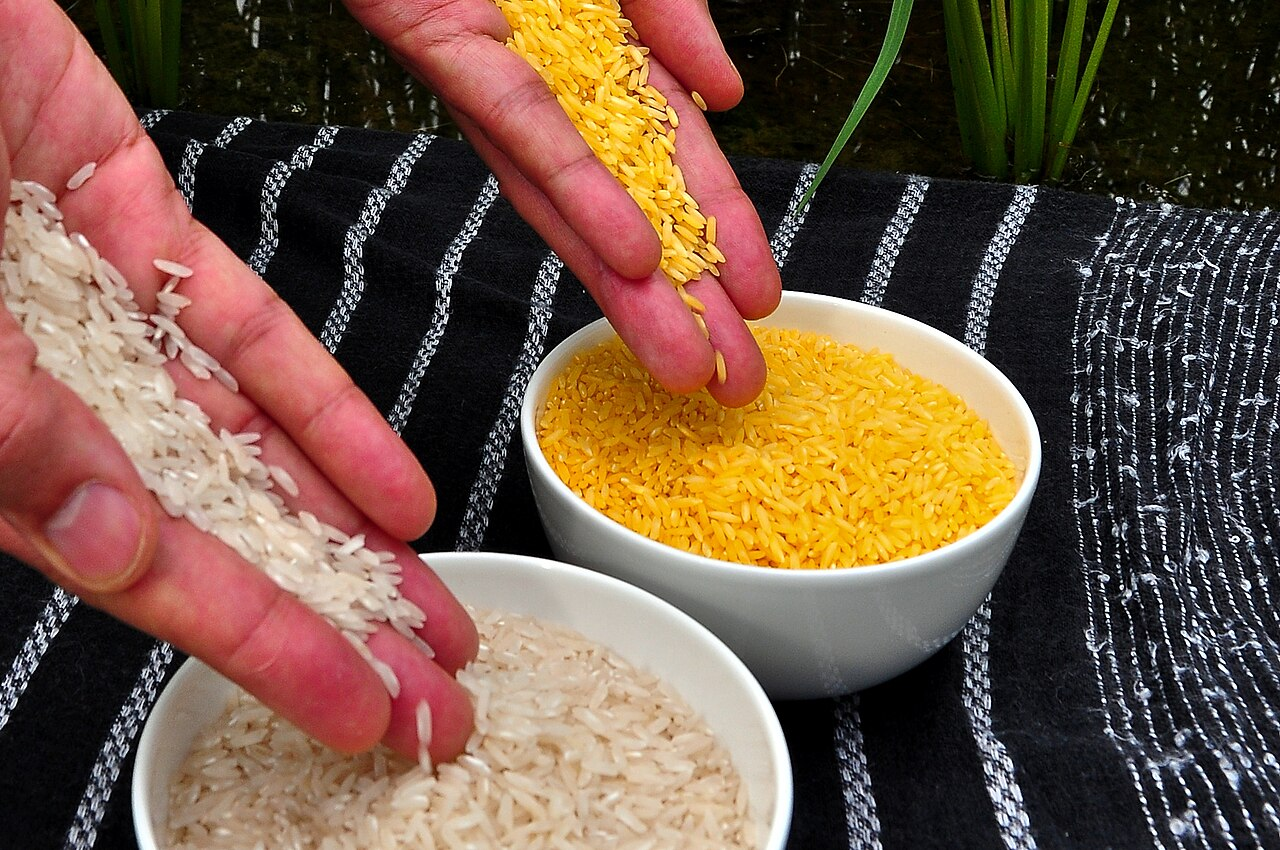
\includegraphics[width=0.46\linewidth]{images/book5/golden-rice-irri.jpg}

{\small Arroz comum e Arroz Dourado. O grão amarelo produz
$\beta$-caroteno em seu endosperma a partir de dois genes acrescentados
da via dos carotenoides. À direita: os dois arrozes comparados no
Instituto Internacional de Pesquisa do Arroz (IRRI, CC~BY~2.0).}
\end{omfigure}

\begin{remark}[O debate]\label{rem:b3:genetic-engineering:gmo}
Trinta anos de cultivo em centenas de milhões de hectares, e cada
revisão sistemática feita pelas academias científicas, não encontraram
efeito sobre a saúde dos cultivos \omterm{def:b3:genetic-engineering:transgenic}{transgênicos} aprovados que difira do
de suas contrapartes convencionais; o transgene é mais um gene entre
quarenta mil, e a proteína que ele produz é testada como qualquer
aditivo alimentar. As questões reais são ecológicas e econômicas: a
propagação de resistência em pragas e ervas daninhas sob seleção
uniforme, o fluxo gênico para parentes silvestres, a concentração do
mercado de sementes e quem se beneficia. São as questões que qualquer
tecnologia agrícola poderosa levanta, e as respostas dependem da
característica e do contexto, não do método pelo qual o gene foi
movido.
\end{remark}

\section{Editar genomas}

\begin{definition}[CRISPR--Cas9]\label{def:b3:genetic-engineering:crispr}
\index{CRISPR}\index{Cas9}\index{RNA-guia}\index{PAM}\index{edição de genomas}
As bactérias guardam fragmentos dos genomas dos fagos que infectaram
seus ancestrais num arranjo de repetições (\emph{CRISPR}),
transcrevem-nos em RNAs-guia curtos e os usam para dirigir uma nuclease
ao corte de qualquer DNA correspondente que entre na célula: um sistema
imune adaptativo com memória genética. Em \emph{Streptococcus pyogenes}
a nuclease é a proteína única \emph{Cas9}, que se liga a um RNA-guia e
a um segundo RNA pequeno, procura no DNA um \emph{\omterm{def:b3:bioinformatics:motif}{motivo} adjacente ao
protoespaçador} de três bases (PAM, 5$'$-NGG), desenrola o DNA
adjacente e, se as vinte bases ao lado do PAM parearem com o guia,
corta as duas fitas a três bases do PAM. Jinek, Charpentier, Doudna e
colaboradores (2012) fundiram os dois RNAs num único \emph{RNA-guia
único} e mostraram que a Cas9 com um guia de sequência qualquer corta o
DNA naquela sequência num tubo de ensaio; em menos de um ano o par já
funcionava em células humanas, de camundongo, de peixe-zebra, de planta
e de levedura. A \emph{edição de genomas} é o que a célula faz com o
corte: a junção de extremidades deixa uma pequena inserção ou deleção
que rompe o gene (um \omterm{def:b3:genetic-engineering:transgenic}{nocaute} numa única etapa, em qualquer organismo,
em semanas), e a \omterm{def:b3:dna-repair:dsb}{recombinação homóloga} com um molde fornecido escreve
ali uma sequência escolhida.
\end{definition}

\begin{omfigure}
\begin{tikzpicture}[every node/.style={font=\scriptsize}, >=stealth]
  % Cas9 outline (drawn first so labels stay on top)
  \draw[thick, omExo, fill=omExo!15] (5.9,1.1) ellipse (2.6 and 1.6);
  \node[omExo!60!black] at (7.7,2.3) {Cas9};
  % target DNA
  \draw[very thick, omDef] (0,0.3) -- (11,0.3); \draw[very thick, omDef] (0,-0.1) -- (11,-0.1);
  % PAM
  \fill[omProp!60] (7.2,-0.2) rectangle (7.9,0.4); \node[below] at (7.55,-0.25) {PAM (NGG)};
  % protospacer
  \draw[omThm, very thick] (4.2,0.5) -- (7.15,0.5); \node[above] at (5.7,0.55) {alvo de 20 bases, pareado com o guia};
  % guide RNA
  \draw[very thick, omMeth!70!black] (4.2,0.3) .. controls (4.2,1.6) and (5.0,1.9) .. (5.4,1.9) -- (6.6,1.9) .. controls (7.0,1.9) and (7.2,2.5) .. (6.8,2.8) .. controls (6.3,3.1) and (5.8,2.7) .. (6.1,2.4);
  \node[left, omMeth!70!black, align=right] at (3.2,2.2) {RNA-guia único:\\20 bases de escolha\\+ grampo de ligação à Cas9};
  % cut
  \draw[omThm, very thick, ->] (6.25,-0.7) -- (6.25,0.35); \node[omThm, below] at (6.25,-0.7) {quebra de fita dupla, a 3 bases do PAM};
  % outcomes
  \draw[->, thick] (2.0,-1.3) -- (2.0,-1.9); \node[below, align=center] at (2.0,-1.9) {junção de extremidades:\\pequena inserção ou deleção\\$\Rightarrow$ mudança de fase, nocaute};
  \draw[->, thick] (10.0,-1.3) -- (10.0,-1.9); \node[below, align=center] at (10.0,-1.9) {recombinação com um\\molde fornecido\\$\Rightarrow$ mudança precisa};
\end{tikzpicture}

{\small A \omterm{def:b3:genetic-engineering:crispr}{Cas9} e seu guia. A proteína liga um \omterm{def:b3:genetic-engineering:crispr}{PAM}, desenrola o DNA ao
lado dele e corta se as vinte bases parearem com o \omterm{def:b3:genetic-engineering:crispr}{RNA-guia}. A quebra é
reparada ou por junção de extremidades, que rompe o gene, ou por
recombinação com um molde, que o reescreve.}
\end{omfigure}

\begin{proposition}[Editar sem quebra]\label{prop:b3:genetic-engineering:editors}
\index{editor de bases}\index{editor prime}\index{fora do alvo}
Cortar as duas fitas é a edição mais grosseira: o desfecho da junção de
extremidades é aleatório, e uma quebra em outro lugar --- um sítio
\emph{\omterm{prop:b3:genetic-engineering:editors}{fora do alvo}}, que difere do guia em algumas posições e que a
\omterm{def:b3:genetic-engineering:crispr}{Cas9} tolera --- é uma mutação que ninguém pediu. Uma \omterm{def:b3:genetic-engineering:crispr}{Cas9} com um
domínio nuclease inativado corta uma só fita; com os dois inativados
ela apenas se liga, e pode levar outras enzimas até uma sequência. Os
\emph{\omterm{prop:b3:genetic-engineering:editors}{editores de bases}} fundem uma \omterm{def:b3:genetic-engineering:crispr}{Cas9} cortadora de uma fita a uma
desaminase que converte C em U (lido como T) ou A em I (lido como G) na
fita desenrolada, mudando uma base sem quebra e sem molde; os
\emph{\omterm{prop:b3:genetic-engineering:editors}{editores prime}} carregam uma transcriptase reversa e um guia
estendido com a sequência desejada, e copiam essa sequência para dentro
da fita cortada, o que permite qualquer substituição e pequenas
inserções ou deleções. A atividade \omterm{prop:b3:genetic-engineering:editors}{fora do alvo} é reduzida por
variantes de \omterm{def:b3:genetic-engineering:crispr}{Cas9} de alta fidelidade, entregando a enzima brevemente
como proteína em vez de gene, e escolhendo guias cujos parentes
genômicos mais próximos difiram em várias posições; ela é medida
sequenciando os sítios previstos e por métodos não enviesados que
captam toda quebra no genoma.
\end{proposition}

\begin{example}[Uma cura]\label{ex:b3:genetic-engineering:sickle}
A doença falciforme é uma única troca de base na $\beta$-globina. A
hemoglobina fetal, feita de $\gamma$-globina, a substituiria, mas os
genes $\gamma$ são desligados depois do nascimento pelo repressor
BCL11A. A primeira terapia \omterm{def:b3:genetic-engineering:crispr}{CRISPR} aprovada (2023) toma as
células-tronco do sangue do próprio paciente, corta com a \omterm{def:b3:genetic-engineering:crispr}{Cas9} o
intensificador eritroide do \emph{BCL11A} para que a junção de
extremidades o inutilize na maioria das células, e devolve as células
depois que a medula do paciente foi esvaziada: as hemácias que elas
produzem são ricas em hemoglobina fetal, não falcizam, e as crises
cessam. A edição é somática --- a linhagem germinativa fica intocada e a
mudança não é herdada --- e usa o desfecho ``grosseiro'', a ruptura,
justamente onde a ruptura é o que se quer.
\end{example}

\begin{theorem}[Propagação super-mendeliana de um impulsor gênico]\label{thm:b3:genetic-engineering:drive}
\index{impulsor gênico}
Um \emph{\omterm{thm:b3:genetic-engineering:drive}{impulsor gênico}} é uma construção que codifica a \omterm{def:b3:genetic-engineering:crispr}{Cas9} e um
guia que corta o alelo selvagem em seu próprio loco num heterozigoto; o
reparo por recombinação copia o impulsor para o cromossomo cortado, de
modo que uma fração $c$ dos gametas do heterozigoto carrega o impulsor
em vez da metade mendeliana. Se o impulsor tem frequência $p$ numa
população grande e de acasalamento aleatório, e não tem custo de
adequação, sua frequência na geração seguinte é
\[
p' = p + c\,p\,(1 - p),
\]
de modo que ele se propaga a partir da raridade a uma taxa proporcional
a $c$ e alcança metade da população em cerca de
$\ln(1/p_{0})/\ln(1 + c)$ gerações a partir de uma frequência inicial
$p_{0}$.
\end{theorem}
\begin{proof}
O acasalamento aleatório dá homozigotos para o impulsor à frequência
$p^{2}$, heterozigotos a $2p(1-p)$ e homozigotos selvagens a
$(1-p)^{2}$. Os homozigotos transmitem o impulsor a todos os seus
gametas, os heterozigotos a uma fração $(1 + c)/2$ (metade por Mendel,
mais $c$ vezes a metade selvagem convertida), e os selvagens a nenhum.
Logo, $p' = p^{2} + 2p(1-p)(1+c)/2
= p^{2} + p(1-p) + c\,p(1-p) = p + c\,p(1-p)$. Para $p$ pequeno isso é $p' \approx (1+c)p$, um crescimento
geométrico de razão $1 + c$, que alcança $1/2$ a partir de $p_{0}$ após
cerca de $\ln(1/2p_{0})/\ln(1+c)$ gerações; o termo logístico só o
desacelera perto do fim.
\end{proof}

\begin{omfigure}
\begin{tikzpicture}
\begin{axis}[
  width=0.7\linewidth, height=5.6cm,
  axis x line=bottom, axis y line=left,
  xmin=0, xmax=20, ymin=0, ymax=1.05,
  xlabel={geração}, ylabel={frequência do impulsor $p$},
  xlabel style={font=\small, at={(axis description cs:0.5,-0.12)}, anchor=north},
  ylabel style={font=\small},
  tick label style={font=\small}, xtick={0,5,10,15,20}, ytick={0,0.5,1},
  clip=false,
]
\addplot[very thick, omThm, mark=*, mark size=1.2pt] coordinates {(0,0.01) (1,0.0189) (2,0.0356) (3,0.0665) (4,0.1224) (5,0.2191) (6,0.3731) (7,0.5836) (8,0.8023) (9,0.9451) (10,0.9918) (11,0.9991) (12,1.0) (13,1.0) (14,1.0) (15,1.0) (16,1.0) (17,1.0) (18,1.0) (19,1.0) (20,1.0)};
\addplot[very thick, omDef, mark=*, mark size=1.2pt] coordinates {(0,0.01) (1,0.015) (2,0.0223) (3,0.0332) (4,0.0493) (5,0.0727) (6,0.1064) (7,0.154) (8,0.2191) (9,0.3047) (10,0.4106) (11,0.5316) (12,0.6561) (13,0.769) (14,0.8578) (15,0.9188) (16,0.9561) (17,0.9771) (18,0.9883) (19,0.9941) (20,0.997)};
\addplot[very thick, gray, dashed, domain=0:20, samples=2] {0.01};
\node[font=\scriptsize, omThm, anchor=south east] at (axis cs:6.5,0.62) {$c = 0.9$};
\node[font=\scriptsize, omDef, anchor=north west] at (axis cs:12.5,0.62) {$c = 0.5$};
\node[font=\scriptsize, gray, anchor=south west] at (axis cs:12,0.02) {mendeliano, $c = 0$: fica em $p_{0}$};
\end{axis}
\end{tikzpicture}

{\small Um \omterm{thm:b3:genetic-engineering:drive}{impulsor gênico} liberado a um por cento, com eficiência de
conversão $0.9$ ou $0.5$ e sem custo de adequação. Um alelo mendeliano
sem vantagem ficaria em um por cento; o impulsor domina em dez ou vinte
gerações.}
\end{omfigure}

\begin{remark}[O que se pode editar]\label{rem:b3:genetic-engineering:ethics}
Editar as células somáticas de um paciente que consente é medicina,
julgada como qualquer tratamento por seus riscos e benefícios. Editar a
linhagem germinativa --- um embrião, cujo descendente carregaria a
mudança --- é diferente em natureza: a pessoa afetada não pode
consentir, a mudança é herdada, e os desfechos \omterm{prop:b3:genetic-engineering:editors}{fora do alvo} e em
mosaico da técnica ainda não estão controlados; depois que um cientista
chinês anunciou, em 2018, tê-lo feito em gêmeas, as academias
científicas da maioria dos países pediram uma moratória e vários
Estados criminalizaram a prática. Um \omterm{thm:b3:genetic-engineering:drive}{impulsor gênico} liberado numa
população silvestre é uma decisão tomada por todos os que vêm depois, e
é por isso que as próprias propostas da área para eliminar os mosquitos
da malária acoplam os impulsores a salvaguardas --- impulsores de
reversão, projetos autolimitados --- e ao consentimento público dos
países envolvidos.
\end{remark}

\section{Exercícios}

\begin{exercise}[$\star$]\label{exo:b3:genetic-engineering:1}
Liste os três componentes que um \omterm{def:b3:genetic-engineering:tools}{plasmídeo} de clonagem precisa ter e
explique a finalidade de cada um.
\end{exercise}

\begin{exercise}[$\star$]\label{exo:b3:genetic-engineering:2}
A EcoRI reconhece GAATTC. Com que frequência o sítio ocorre, em média,
em DNA aleatório, e quantos fragmentos ele faz do genoma de
\qty{4.6}{Mb} de \emph{E.~coli}? Por que o número real é um pouco
diferente?
\end{exercise}

\begin{exercise}[$\star$]\label{exo:b3:genetic-engineering:3}
Enuncie as três etapas de temperatura de um ciclo de PCR e o que
acontece em cada uma. Por que a polimerase precisa ser termoestável?
\end{exercise}

\begin{exercise}[$\star$]\label{exo:b3:genetic-engineering:4}
De que a \omterm{def:b3:genetic-engineering:crispr}{Cas9} precisa para cortar uma dada sequência, e que dois
desfechos podem seguir-se ao corte?
\end{exercise}

\begin{exercise}[$\star\star$]\label{exo:b3:genetic-engineering:5}
Uma PCR roda $35$ ciclos com eficiência $E = 0.9$ a partir de $50$
cópias. Quantas cópias resultam? Uma qPCR de duas amostras dá
$C_{T} = 18.2$ e $25.5$; com $E = 0.95$, qual é a razão entre suas
quantidades iniciais?
\end{exercise}

\begin{exercise}[$\star\star$]\label{exo:b3:genetic-engineering:6}
Por que se usa uma biblioteca de cDNA, e não uma biblioteca genômica,
para expressar uma proteína humana em bactérias? Nomeie dois outros
obstáculos a fazer uma proteína humana em \emph{E.~coli} e diga como
cada um é superado.
\end{exercise}

\begin{exercise}[$\star\star$]\label{exo:b3:genetic-engineering:7}
Um camundongo \omterm{def:b3:genetic-engineering:transgenic}{nocaute} é feito por \omterm{def:b3:genetic-engineering:transgenic}{direcionamento gênico} em
células-tronco embrionárias. Explique por que o primeiro camundongo
nascido é uma quimera, por que é preciso cruzá-lo, e que fração dos
netos de uma quimera cuja linhagem germinativa é metade direcionada são
\omterm{def:b3:genetic-engineering:transgenic}{nocautes} homozigotos se os avós heterozigotos forem intercruzados.
\end{exercise}

\begin{exercise}[$\star\star$]\label{exo:b3:genetic-engineering:8}
Escolhe-se um \omterm{def:b3:genetic-engineering:crispr}{RNA-guia} de 20 bases com um \omterm{def:b3:genetic-engineering:crispr}{PAM} NGG. Quantos sítios de um
genoma de $3.2\times 10^{9}$ bp (as duas fitas) correspondem ao guia
exatamente por acaso? Quantos correspondem com até duas discordâncias,
se a \omterm{def:b3:genetic-engineering:crispr}{Cas9} as tolera? (Conte as sequências a até duas discordâncias como
$1 + 3\binom{20}{1} +
9\binom{20}{2}$.)
\end{exercise}

\begin{exercise}[$\star\star$]\label{exo:b3:genetic-engineering:9}
Usando o \cref{thm:b3:genetic-engineering:drive}, calcule a frequência
de um impulsor com $c = 0.8$ após três gerações a partir de
$p_{0} = 0.05$, e estime o número de gerações para alcançar $0.5$.
\end{exercise}

\begin{exercise}[$\star\star\star$]\label{exo:b3:genetic-engineering:10}
A terapia da doença falciforme rompe um intensificador em vez de
corrigir a mutação da $\beta$-globina. Dê duas razões pelas quais a
ruptura por junção de extremidades foi escolhida em vez da correção por
\omterm{def:b3:dna-repair:dsb}{recombinação homóloga} em células-tronco do sangue, e uma desvantagem.
\end{exercise}

\begin{exercise}[$\star\star\star$]\label{exo:b3:genetic-engineering:11}
Um \omterm{thm:b3:genetic-engineering:drive}{impulsor gênico} contra um mosquito tem custo de adequação $s$ nos
homozigotos. Modifique a recorrência para incluir a seleção contra os
homozigotos do impulsor e determine a condição sobre $c$ e $s$ para que
o impulsor se propague a partir da raridade. Depois explique por que os
alelos de resistência --- produtos de junção de extremidades no alvo que
o guia já não reconhece --- são o principal obstáculo na prática.
\end{exercise}

\begin{exercise}[$\star\star\star$]\label{exo:b3:genetic-engineering:12}
Argumente, com os mecanismos deste capítulo e do
\cref{ch:b3:dna-repair}, por que a edição germinativa de um embrião
humano não consegue hoje garantir o desfecho pretendido em cada célula,
e que evidência seria necessária antes que uma pessoa racional pudesse
considerá-la segura.
\end{exercise}

\section{Problema: de um gene a um fármaco e a uma lavoura}

\begin{problem}[{Problema de fim de semana --- um gene clonado com a
aritmética dos sítios de restrição e da transformação, um vírus contado
por qPCR, um hormônio produzido às toneladas num fermentador, um genoma
editado com seus efeitos fora do alvo contados e um impulsor gênico
cronometrado, terminando nas cópias de um vírus numa amostra, no volume
anual de fermentador para a insulina do mundo e no número de gerações
de que um impulsor precisa}]
\label{pb:b3:genetic-engineering:1}
Dados: um gene de \qty{1.5}{kb}; um sítio de restrição de seis bases;
um \omterm{def:b3:genetic-engineering:tools}{plasmídeo} de \qty{4}{kb}; eficiência de transformação de
$2\times 10^{7}$ colônias por micrograma de \omterm{def:b3:genetic-engineering:tools}{plasmídeo}; a ligação dá
inserto a \qty{10}{\%} dos \omterm{def:b3:genetic-engineering:tools}{plasmídeos}. Eficiência da qPCR $E = 1$,
limiar $N_{T} = 10^{12}$. Insulina: \qty{5.8}{kDa}, um paciente usa
$40$ unidades por dia, sendo uma unidade \qty{35}{\micro g}; $10^{7}$
pacientes; um fermentador rende \qty{2}{g/L} de produto por lote, dez
lotes por ano. Genoma $3.2\times
10^{9}$ bp. Conversão do impulsor
$c = 0.9$, liberado a $p_{0} = 0.001$.

\medskip
\noindent\textbf{Parte I --- Clonagem.}
\begin{enumerate}
  \item Com que frequência um dado sítio de seis bases ocorre em DNA
        aleatório? Qual é a probabilidade de o gene de \qty{1.5}{kb}
        não conter nenhum sítio desses, de modo que a enzima possa ser
        usada para cloná-lo inteiro?
  \item Se ele contiver um sítio, como você o clonaria mesmo assim?
        (Dois métodos.)
  \item \qty{100}{ng} de \omterm{def:b3:genetic-engineering:tools}{plasmídeo} ligado são transformados. Quantas
        colônias, e quantas carregam o inserto?
  \item Usa-se a triagem azul--branco. Que fração das colônias é
        branca, e quantas colônias brancas é preciso pescar para ter
        \qty{99}{\%} de chance de ao menos uma carregar o gene na
        orientação certa (metade dos insertos)?
  \item O \omterm{def:b3:genetic-engineering:tools}{plasmídeo} recombinante tem \qty{5.5}{kb}. Uma célula contém
        $50$ cópias e se divide a cada \qty{30}{min}. Depois de um
        crescimento de uma noite (\qty{16}{h}) a partir de uma célula,
        quantas moléculas de \omterm{def:b3:genetic-engineering:tools}{plasmídeo} e que massa de DNA plasmidial
        (\qty{650}{Da} por par de bases)?
  \item Por que o \omterm{def:b3:genetic-engineering:tools}{plasmídeo} precisa de uma origem bacteriana, ao passo
        que o gene humano inserido não precisa de promotor bacteriano
        para a clonagem, mas precisa para a expressão?
\end{enumerate}

\medskip
\noindent\textbf{Parte II --- Contar um vírus.}
\begin{enumerate}[resume]
  \item A amostra de um paciente cruza o limiar em $C_{T} = 28$.
        Quantas cópias havia na reação? E outra em $C_{T} = 35$?
  \item Sensibilidade: quantos ciclos são necessários para levar uma
        única cópia ao limiar?
  \item O ponto de corte do teste é fixado em $C_{T} = 38$. A que
        número de cópias isso corresponde, e por que não usar $45$
        ciclos?
  \item Uma molécula contaminante do produto de uma corrida anterior
        entra numa amostra negativa. Em que ciclo ela cruza o limiar?
        Que prática de laboratório impede isso?
  \item A transcrição reversa converte \qty{40}{\%} do RNA viral em
        DNA. Corrija a contagem da questão 7 para a primeira amostra.
  \item Duas amostras diferem em $\Delta C_{T} = 3.3$ com $E = 1$, mas
        a eficiência é na verdade $0.9$. Que diferença em vezes o
        analista relata, e qual é a verdadeira?
\end{enumerate}

\medskip
\noindent\textbf{Parte III --- Insulina às toneladas.}
\begin{enumerate}[resume]
  \item Calcule a massa diária de insulina por paciente e a necessidade
        anual do mundo para $10^{7}$ pacientes, em quilogramas.
  \item Quantos mols de insulina são esses, e quantas moléculas?
  \item Que volume de fermentador, rodado dez lotes por ano, produz
        isso? Compare com uma piscina de \qty{2500}{m^3}.
  \item A extração de glândulas dava \qty{1}{kg} de insulina por
        \qty{8000}{kg} de pâncreas; um pâncreas de porco pesa
        \qty{100}{g}. De quantos porcos por ano o mundo precisaria?
  \item Por que o hormônio recombinante é preferido mesmo onde a
        insulina animal é barata? Dê duas razões.
  \item Os análogos de insulina diferem da sequência humana em um ou
        dois resíduos. Explique por que um análogo ainda é um fármaco
        que age sobre o receptor humano, e por que a troca de um
        resíduo pode alterar seu tempo de dissociação.
\end{enumerate}

\medskip
\noindent\textbf{Parte IV --- Editar e impulsionar.}
\begin{enumerate}[resume]
  \item Quantas correspondências exatas de um guia de 20 bases mais NGG
        o genoma contém por acaso (as duas fitas: $6.4\times 10^{9}$
        posições)?
  \item Se a \omterm{def:b3:genetic-engineering:crispr}{Cas9} tolera até três discordâncias, quantas sequências
        estão a até três discordâncias do guia, e quantos sítios \omterm{prop:b3:genetic-engineering:editors}{fora
        do alvo} de acaso daí resultam?
  \item As células-tronco do sangue editadas são $10^{7}$;
        \qty{80}{\%} carregam a ruptura pretendida. Quantas células
        carregam uma quebra \omterm{prop:b3:genetic-engineering:editors}{fora do alvo} num dado sítio, se ele é
        cortado numa célula em $10^{4}$, e por que uma quebra num gene
        supressor de tumor numa única célula-tronco é motivo de
        preocupação?
  \item Calcule a frequência do impulsor após $1, 2, 3$ gerações a
        partir de $p_{0} = 0.001$, e estime as gerações até $0.5$.
  \item Um mosquito tem dez gerações por ano. Quantos anos para
        dominar? Como um custo de adequação de \qty{20}{\%} nos
        homozigotos muda o quadro qualitativamente?
  \item Um alelo de resistência surge quando a junção de extremidades,
        e não a recombinação, repara o corte, com probabilidade
        $1 - c = 0.1$ por tentativa de conversão. Estime o número de
        alelos de resistência criados numa população de $10^{6}$
        heterozigotos em uma geração, e explique o que acontece com o
        impulsor se eles forem aptos.
  \item Resuma: as cópias na primeira amostra (questão~7), o volume
        anual de fermentador para a insulina do mundo (questão~15) e as
        gerações para o impulsor alcançar metade da população
        (questão~22).
\end{enumerate}
\end{problem}
